%
% 2017 by Michal Young
% based heavily on Cool manuals by Aiken and Boyland
% revised September 2018
% 
%
\documentclass[11pt]{article}

\usepackage{fontspec,lipsum}
\defaultfontfeatures{Ligatures=TeX}
\setromanfont{Minion Pro}
\setsansfont{Myriad Pro}


% \usepackage{alltt}
\usepackage{verbatim}
\usepackage{grammar}
\usepackage{semantic}

\usepackage{url}
\usepackage{graphicx}

\usepackage{amssymb}
\usepackage{quackman}

% Actual margin is 1.5 in + this number
\topmargin -.5in

% Text height:
\textheight 9in


\begin{document}


\title{Quack:  A Language for Novice Compiler Writers\\
\small   Version 0.3.3,, September 22, 2018}

\author{Michal Young}
\date{ }
\maketitle

\tableofcontents 
\clearpage

\section{Introduction}

\begin{quotation}
\noindent
quack (noun)\\
1. charlatan\\
2. a pretender to medical skill\\
3. a cry made by a duck
\begin{flushright}
-- \em Merriam-Webster Dictionary
\end{flushright}
\end{quotation}

This manual describes a small language defined
specifically for use  
in a very short (10 week) compiler construction class.  Quack is an
object-oriented language with single inheritance and flow-insensitive
type inference.  To make it
viable for a 10 week course, Quack
purposely omits many features, such as templates (generics),  
arrays, and overloading,  that require more sophistication in the type system and code
generation.   Nonetheless I believe implementing Quack will deepen your
understanding of the languages and compilers you use regularly. 


\subsection{How to Read This Manual}

Do not expect to absorb everything here in one reading.   Give it a
light reading once, then re-read parts relevant to the part of the
project you are working on.  In the first week, you will need to
understand the \emph{lexical}
structure of Quack to build your scanner (also called a ``lexer'').
Shortly after, you will need to understand the \emph{syntactic}
structure of Quack to build a parser, and it will help to understand
the static semantics (type system) and dynamic (that is, execution)
semantics so that you structure your grammar in a way that eases
construction of the abstract syntax tree structure you will need for
type checking and code generation.  You will need to study the type
system more thoroughly to build the abstract syntax tree and the type
checker.   Since the type checking and type inference are basically an
abstraction of execution semantics, the code generation phase will
likely not require any additional understanding of Quack. 


\subsection{A Quick Tour}

\begin{figure}
\verbatiminput{samples/Sqr.qk}
\caption[A simple Quack program]{A simple Quack program 
  that prints 
  ((5,5), (5,10), (10,10), (10,5))} 
\label{fig-square}
\end{figure}

The example program in Figure~\ref{fig-square} illustrates some of the
main features of Quack and should help in understanding the piecemeal
presentation that follows.   This program introduces three Quack
classes (Pt, Rect, and Square) and uses the built-in classes Int and
String.   The output should be 

\begin{verbatim}
((5,5), (5,10), (10,10), (10,5))
\end{verbatim}

Note  that arguments to the constructor for class Pt are given in
the class declaration, and the statements immediately following the
class signature are the body of the constructor.  As in Java, 'this'
is an identifier bound to the current object instance (sometimes
called the ``receiver'' object) in all methods, including the
constructor.  Unlike Java, Quack does not permit omitting 'this' in a
reference to an instance variable.   (If 'this' could be omitted, 
we would need another way to distinguish between instance 
variables and local variables used
only in the constructor.) 

Methods STR and PRINT are defined in Obj, the root of the class
hierarchy, but may be overridden by other classes using the standard
compatibility rules familiar from languages like Java.   Thus if a
method STR (which is roughly like Java's 'to\_string' method) is
defined, it must take no arguments (except the implicit 'this' passed
in all method calls), and it must return a String or a subclass of
String.  Method PRINT is seldom overridden, but o.PRINT() prints 
o.STR, so the behavior of PRINT is affected by overriding STR. 

Note there are no variable declarations in the sample program.
Nonetheless, Quack is a statically typed language like Java, not a
dynamically typed language like Python.  The static type of a variable
is calculated (``inferred'') by the compiler by considering all
assignments to the variable.\footnote{This is also somewhat similar to
  \emph{auto} in C++, but differs in that we consider 
  \emph{all} assignments to the variable rather than only 
  the current assignment.} Thus the instance variables x and y of
Pt have type Int, because they are assigned an Int value.  

While this sample program does not include type declarations for
instance variable or local variables, an assignment can optionally
include a type declaration: 

\begin{verbatim}
a_square: Rect = Square( Pt(3,3), 5 );
\end{verbatim}

If this leaves you wondering what happens when different types are
assigned to the same variable, good for you.  The type inference rules
will be described in more detail later, but for now suffice it to say that
the static type of a variable is the most specific type that is 
consistent with all assignments to that variable


\section{Lexical Structure}
\label{lex-struct}

\subsection{White Space}

White space consists of any sequence of the ASCII characters:
HT, NL, CR, and SP\@.
These characters are represented by the following C/C++ character
literals respectively:  \verb|'\t'|, \verb|'\n'|,
\verb|'\r'|, and \texttt{' '}. 
White space is ignored in Quack, except in quoted strings and to
separate tokens.  

\subsection{Keywords}

The keywords of Quack  are 

\bgroup \bf
\begin{tabular}{lll}
class&def&extends\\
if&elif&else\\
while&return\\
typecase\\
\end{tabular}
\egroup

\noindent 
There are also a handful of predefined identifiers
that name built-in classes and values.  They are not
keywords. The predefined identifiers in Quack are 

\bgroup \bf
\begin{tabular}{lll}
String&Int&Obj\\
Boolean&true&false\\
and&or&not\\
Nothing&none\\
\end{tabular}
\egroup


\subsection{Punctuation}

The following symbols are used like keywords in Quack: 
\begin{description}
\item[$+,-,*,/$]  Arithmetic operators, syntactic sugar for PLUS, MINUS,
  TIMES, DIVIDE method calls. 
\item[$==,  <\,=, <, >=, >$] Comparisons, syntactic sugar for 
   EQUALS, ATMOST, LESS, ATLEAST, MORE. 
\item[and,or,not]  Logical operations with short-circuit semantics. 
   These are not syntactic sugar.  They can be used only for boolean 
   values, and they have short-circuit semantics. 
\item[\{ \}] Used to mark the beginning and end of a class 
   or statement block. 
\item[=] Used to indicate assignment.  I pronounce this symbol
  ``gets''. 
\item[( )] Used to group sub-expressions. 
\item[,] Used to separate formal or actual arguments in an argument
  list.
\item[;] Used to mark the end of a statement. 
\item[.]  Used to reference a method or variable in an object. 
\item[:] Used to associate a type with a variable in an assignment
    and to indicate the type of value returned by a method. 
\end{description}


\subsection{Identifiers}

Identifiers are strings (other than keywords) beginning with a letter
or underscore and consisting of letters,
digits, and the underscore character.  \verb|my_cool_fUNCtion|  is a  
an identifier, as are \verb|l33tc0de|, and \verb|___just__dont|.  Note
that PLUS, MINUS, TIMES, and DIVIDE are valid identifiers and can
appear as method names in any class to give meaning to the binary
operators \(+, -, *\) and \(/\).  Likewise EQUALS, ATMOST, ATLEAST, 
LESS, and MORE can be defined so that the comparisons 
\(== , <\,=, <, >=, > \) work for some class. 
Using those operators on values for
which they are not defined results in the same error messages as using
any other method that has not been defined.  (Nothing prevents you
from defining a comparison method from returning a non-boolean value,
but it's a bad idea.) 


Although it is conventional to begin class names with a capital letter
and variable and method names with lower case letters, it is not a
rule of Quack.  In lieu of adding a \emph{properties} facility to
Quack, I  have informally adopted the convention of starting
a `getter' method name with a single underscore.  

\subsection{Integer Literals} 

Integer literals are non-empty strings of digits. \verb|0| is an integer
literal, as are \verb|42|,  \verb|99099|, and \verb|00088|.
\verb|-99| is not an integer literal; it is a pair of tokens, the
second of which is the integer literal \verb|99|.  \footnote{Do you
  see why -99 is not an integer literal?  Consider the expression $b-99$.}


\subsection{String Literals}

There are two forms for string literals.
The simple version of
string literals are enclosed in double quotes {\tt "\ldots"}.  Within a string literal, a
sequence `\texttt{\char92$c$}' is illegal unless it is one of
the following: 
\begin{quote}
\begin{tabular}{rl}
\texttt{\char92 0} & NUL \\
\texttt{\char92 b} & backspace \\
\texttt{\char92 t} & tab \\
\texttt{\char92 n} & newline \\
\texttt{\char92 r} & return \\
\texttt{\char92 f} & form feed \\
\texttt{\char92 "} & double quote \\
\texttt{\char92 \char92} & backslash
\end{tabular}
\end{quote}

A newline character may not appear in the simple form of a string
literal (even if escaped):
\begin{verbatim}
"This is not\
OK"
\end{verbatim}

Note the difference between the illegal example above, in which the newline
character itself is escaped, and the following, in which the newline
character is denoted by an escape code: 

\begin{verbatim}
"This is\n OK"
\end{verbatim}


The other form of string literals starts with \emph{three} double
quotes and continues until ended by three double quotes (again).
Any characters, including backslashes and newlines are legal.
The only thing forbidden is three double quotes.  Thus the following
represents a string literal:
\begin{verbatim}
"""This starts a string literal
that continues on for several lines
even though it includes "'s and \'s and newline characters
in a "wild" profu\sion\\ of normally i\\egal t"ings.\"""
\end{verbatim}
The string contains literally everything inside of it. 

\subsection{Comments}

There are two forms for comments in Quack.  Any characters after two
slashes \verb"//" and before the next newline (or EOF, if there is no next
newline) are ignored. Also, any characters excepting the sequence
\verb|*/| may be enclosed in C-style comments: \verb|/*|\ldots\verb|*/|.

. 

\section{Quack Grammar}

\subsection{Notation}

The grammar of Quack is described here informally in English and more
formally in an extended BNF\footnote{Backus Normal Form, or
  Backus-Naur Form, depending on whom you ask.} notation. 

\begin{description}
\item[\literal{foo}] denotes the literal string  ``foo''.
  We use this for keywords like \literal{class} and punctuation 
  like \literal{:}.  
\item[\nonterminal{Sym}] (capitalized, in angle brackets) indicates $Sym$ is a non-terminal symbol. 
  For example, \nonterminal{Class} represents the grammatical symbol
  for a class in Quack, but \literal{class} denotes the keyword that 
  introduces a class definition. 
\item{\terminal{t}} (italic font, lower case) indicates $t$ is a terminal symbol (other than 
  a keyword or punctuation).  For example, \terminal{ident} 
  is the terminal symbol for an identifier in Quack.  ``foo'' and 
  ``a\_long\_variable\_name'' are two different identifiers in Quack,
  both represented by \terminal{ident} in the grammar.
\end{description}


We use the following shorthands and conventions in our EBNF: 

\begin{bullets}

\item We use $\lambda$ to represent the empty string.  
This is just for clarity of expression. 

\item  We use a postfix star (*) to denote zero or more repetions (exactly like
  Kleene star in a regular expression).\footnote{An alternative EBNF
    convention you will sometimes encounter is to use curly braces \{
    \ldots \} to enclose a phrase that can be repeated.   Although the
    braces notation is very readable, it was not practical to use
    braces in this way in parser generator tools that used braces for
    other purposes.  Moreover, it is desirable to be as consistent as
    possible between our notation for regular expressions and our
    notation for context-free grammars. Thus we adopt the Kleene star
    notaton.}  

\begin{grammar}
\nonterminal{S} & \(\alpha\)  \kleene{ X Y Z }  \(\beta\)
\end{grammar}

indicates that $X Y Z$ may appear zero or more times between $\alpha$
and $\beta$. 

\item We use square braces like \optional{ X Y Z}  to indicate an optional sequence of
  symbols, i.e., zero or one occurrences. 

\item We use parentheses to group symbols. 

\end{bullets}

\subsection{Structure of a Quack program}

A program is a sequence of zero or more class definitions followed by zero or
more statements. 

\begin{grammar}
\nonterminal{Program} &
    \kleene{\nonterminal{Class}}
    \kleene{\nonterminal{Statement}} 
\end{grammar}

A class is a class signature followed by the body of the class.  The
class signature gives the class name, arguments to its constructor
method,  and its superclass.  

\begin{grammar}
\nonterminal{Class} & \nonterminal{Class\_Signature}
\nonterminal{Class\_Body}\\[1ex]
\nonterminal{Class\_Signature} & 
  \literal{class} \terminal{ident}  
  \literal{(} \nonterminal{Formal\_Args} \literal{)}
  \optional{ 
      \literal{extends} \terminal{ident}
   }\\
\nonterminal{Formal\_Args} & 
    \optional{ \terminal{ident} \literal{:} \terminal{ident} 
         \kleene{ \literal{,}  \terminal{ident} \literal{:}
           \terminal{ident}  }
     }
\end{grammar}

\noindent For example, 
\begin{verbatim}
class Point(x: Int, y: Int) extends Obj
\end{verbatim}

When the \verb|extends| clause is omitted, it is taken as 
shorthand for \verb|extends Obj|, so the above example may be
rewritten 
\begin{verbatim}
class Point(x: Int, y: Int)
\end{verbatim}


Classes in Quack form an inheritance hierarchy which is also a type
hierarchy.  This is familiar from languages like Java:  If class $C$
is a subclass of class $S$, then type $C$ is also a subtype of type
$S$ and an object of type $C$ may be used where an object of type $S$
is required.   When a subclass introduces a method that overrides a
method of its superclass, the usual rules of contravariance for method arguments and
covariance for results apply.   Obj is the root of the class
hierarchy.  

Classes may not be redefined.  Identifiers in Quack, including class
names, are case sensitive; MyClass is different from myclass which is
different from myClass.  Although we conventionally use capitalized
identifiers for class names in Quack, it is not a rule of the
language.  

Class signatures have global scope.  All methods are accessible
through objects of that class (i.e., like public methods in Java or C++), but
all instance variables are accessible only within a class (like
private fields in Java or C++).  There is no identifier overloading in
Quack: Although two things with the same name may appear in distinct
scopes,  a class cannot have the same name as a method or
variable.  The convention of capitalizing class names and using
lowercase for variables and methods will prevent clashes between
them. 

The body of a class begins with a sequence of zero or more statements
that act as the constructor of the class.  All instance variables must
be created in these statements.  Method declarations follow the
statements.  

\begin{grammar}
\nonterminal{Class\_Body} & {\EnterBlock} 
  \kleene{\nonterminal{Statement}}
  \kleene{\nonterminal{Method}}
  {\LeaveBlock}
\end{grammar}

Method declarations require explicit declarations of argument and
result types.  This makes type checking or type inference simple and
local. 

\begin{grammar}
\nonterminal{Method} & 
    \literal{def} \terminal{ident} 
    \literal{(} \nonterminal{formal\_arguments} \literal{)} 
   \optional{ 
     \literal{:} \terminal{ident}  
   } \newline
   \nonterminal{Statement\_Block}
\end{grammar}


\noindent A statement block is a sequence of zero of more statements,
delimited by curly braces. 

\begin{grammar}
  \nonterminal{Statement\_Block} &
  {\EnterBlock} \kleene{\nonterminal{Statement}} {\LeaveBlock}
\end{grammar}


\section{Classes and Types}

Although the type system of Quack is simple and fairly conventional,
a full description of type checking and inference requires a separate
document.  Here we give a short summary.  Refer to \emph{Type Checking
  and Type Inference for Quack} for details. 

\subsection{Class Hierarchy}

As in many object-oriented programming languages, each class in Quack
is associated with a type of the same name.   Unlike Java or C++, it
is also the case in Quack that every type an object  can
have\footnote{The hedge ``that a variable can have'' is because there
  are two special types, $\top$ and $\bot$, that we use in type
  checking to represent uninitialized variables and
  type errors, respectively.  No object ever has either of these types.}
is a class.

Quack classes have single inheritance.  Every class except \emph{Obj}
has a single super-class.  The superclass of a class is designated by
the \emph{extends} clause of the class declaration, and an omitted
\emph{extends} clause implicitly designates \emph{Obj} as the
superclass.   There are no Java-style interfaces or other
means to create a supertype (subtype) relation that is not also an
inheritance relation.   

The subtype relation is a partial order, and we write $C \le{} S$ to
indicate that C is a subtype of S.  Note that the subtype relation is
reflexive and transitive: $A \le{} B$ and $A \le{} B \land{} B \le{} C
\Rightarrow A \le C$.  Cycles in the subclass relation are
forbidden.  (This is a separate 
check that the Quack compiler must make before attempting type
checking.)   

The subtype relation is intended to satisfy a weak version of the Liskov substitution
principle:  Anywhere an object of type $A$ may legally be used, an
object of type $B$ such that $B \le{} A$ may legally be used.  In
other words, where an object of a given type is expected (e.g., as an
actual argument passed to a method), an object of any subtype of the
expected type is acceptable.     Quack follows the usual covariance
and contravariance rules familiar from other object-oriented
languages like Java, without the complications introduced by collections,
generics, and first-class functions. 

Quack supports a limited version of intraprocedural, flow-insensitive
type inference.  Type checking and type inference are described in a
separate document. 

% \subsection{Type Inference}

% Quack supports a limited version of type inferencing.  Type inference
% in Quack is \emph{intraprocedural} and \emph{flow-insensitive}.
% \emph{Intraprocedural} means that we can perform type checking for
% individual methods one at a time, in any order; we need the
% \emph{signatures} of other methods (in the same class and in other
% classes that the method uses) but we do not need the \emph{bodies} of
% those methods or the results of type checking them.
% \emph{Flow-insensitive} means that we can perform type checking and
% type inference without concern for the order in which statements of
% the method may
% be executed.  There is one exception to this:  Quack requires that a
% variable be initialized before use on every syntactic path, and this
% is a \emph{flow-sensitive} but \emph{path-insensitive} analysis.
% These are fairly standard design choices, often left implicit in
% language reference manuals. 

% Students in the Winter 2017 offering of CIS 461/561 felt that type
% inference was the most challenging part of the project, more difficult
% than code generation and far more difficult than scanning and
% parsing.  The implementation of type inference need not be 
% very complex, but it does require careful design, and being an
% unfamiliar task for most of you it is likely you'll make a few
% mistakes on the way to a complete solution.   
%   I will try to set aside as much time as we can for this
% phase, and suggest tactics for making it as simple as possible,
% but you should anticipate that type inference will be a fairly major
% task. 

\section{Statements}

\subsection{Control structures}

Quack has two control structures, \emph{if} conditionals and
\emph{while} loops.  Conditionals include optional \emph{elif} and
\emph{else} parts.  Note that we avoid the ``dangling else
problem''\footnote{The dangling else problem is a classic grammar
  booboo (I believe that's the technical term) that appears in C and
  many languages that imitate C grammar, such as Java.  Your textbook
  likely discusses it.  You can find a short, clear explanation in
  Wikipedia. Another way to avoid the problem is to close an \emph{if}
  statement with \emph{endif} of a similar exp.  In languages like C and Java, the dangling else problem
  is typically resolved by making an \emph{else} bind to the nearest
  \emph{if}}. 
by making each branch be a block, not a statement.  

\begin{grammar}
\nonterminal{Statement} & 
   ~~\literal{if} \nonterminal{R\_Expr} \nonterminal{Statement\_Block}
   \newline
   \kleene{\literal{elif} \nonterminal{R\_Expr}
     \nonterminal{Statement\_Block}}
   \newline
   \optional{\literal{else} 
     \nonterminal{Statement\_Block}}
\end{grammar}

The only loop construct in Quack is the basic  \emph{while} loop, 
without  \emph{break} or \emph{continue} or any other fancy bits:

\begin{grammar}
\nonterminal{Statement} & 
  \literal{while} \nonterminal{R\_Expr} \nonterminal{Statement\_Block}
\end{grammar}




\subsection{Assignments}

An assignment statement has a left-hand side and a right hand side.
The left hand side evaluates to a \emph{location}.\footnote{You may
  think of a location as a memory address, although it is also useful 
  have a more abstract notion of an \emph{environment} as a map from 
  names to locations and a \emph{store} as a map from locations 
  to values.}
The right hand side evaluates to a \emph{value}.  All values in Quack
are references to objects.  

\begin{grammar}
\nonterminal{Statement} & 
   \nonterminal{L\_Expr} 
   \optional{\literal{:} \terminal{ident}} 
   \literal{=} \nonterminal{R\_Exp} \StmtEnd
\end{grammar}

A left-hand expression (that is, designation of a location in which to
store a value) is often just an identifier, but sometimes it is the
location of a field of an object.  

\begin{grammar}
\nonterminal{L\_Expression} & \terminal{ident}\\
\nonterminal{L\_Expression} &
    \nonterminal{R\_Exp} \literal{.} \terminal{ident}\\
\end{grammar}

It may appear surprising that a right-hand expression, evaluated for
value, can appear as part of a location in a left-hand expressiion,
but consider: 

\begin{verbatim}
foo.findmax(this.children).weight = 42;
\end{verbatim}

Note that field access is left-associative:  a.b.c is (a.b).c, not
a.(b.c).  

\subsection{Bare Expressions}

A right-hand expression by itself can serve as a statement.  This may
make sense if evaluaton of a method  has an \emph{effect} as well
as a \emph{value}.  

\begin{grammar}
\nonterminal{Statement} &  \nonterminal{R\_Exp} \StmtEnd
\end{grammar}

I think allowing all bare expressions as statements is probably a bad
idea, but the grammar is not the place to restrict which expressions
can appear as statements.  Extending the type system so that each 
method either has an effect or a result but never both, and then
restricting bare expressions to method calls with effects, might be a
nice extension project. 

\section{Expressions}

So far we have a lot of  ways to name and structure things, but we haven't
defined any ways to perform actual computation.  It's time to fix that.   In
what follows I'll use `expression' as shorthand for `right-hand
expression' except when necessary to disambiguate. 

\subsection{Constants}

The simplest expressions are literal constants.  The literal constants
in Quack are quoted strings and integers, whose forms are described in
the lexical structure and are completely unsurprising. 

\begin{grammar}
\nonterminal{R\_Expr} & \terminal{string\_literal}\\
\nonterminal{R\_Expr} & \terminal{integer\_literal}
\end{grammar}

Also, anything that can be named in a left-hand expression can be
evaluated in a right-hand expression: 

\begin{grammar}
\nonterminal{R\_Expr} & \nonterminal{L\_Expr}
\end{grammar}

\subsection{Binary Operators}

Quack has a handful of binary operators for addition, subtraction,
etc.  

\begin{grammar}
\nonterminal{R\_Expr} & 
    \nonterminal{R\_Expr} \literal{+} \nonterminal{R\_Expr}\\ 
\nonterminal{R\_Expr} & 
    \nonterminal{R\_Expr} \literal{-} \nonterminal{R\_Expr}\\ 
\nonterminal{R\_Expr} & 
    \nonterminal{R\_Expr} \literal{*} \nonterminal{R\_Expr}\\ 
\nonterminal{R\_Expr} & 
    \nonterminal{R\_Expr} \literal{/} \nonterminal{R\_Expr}\\ 
\nonterminal{R\_Expr}  &
    \literal{-} \nonterminal{R\_Expr}\\ 
\end{grammar}

This expression grammar is highly ambiguous:  How do we know whether
\(a-b+c\) is \(a-(b+c)\) or \((a-b)+c\) ?  It would be
possible to expand the grammar to determine both associativity and
precedence, but we'll keep it simple (and exploit features of almost
all parser generator tools) by simply declaring our intention:
Multiplication and division have higher precedence than addition and
subtraction, and they are all left-associative (i.e., \(a-b+c\) is
\((a-b)+c\) but \(a-b/c\) is \(a-(b/c)\)).   Unary negation has higher
precedence than multiplication and division, so \( a * - b \) is the
same as \( a * (0 - b)\) and \( -a * b\) is the same as 
\( (0-a) * b\). 


If we want to group in a different way, or just be very clear about
the meaning of an expression, we can use parentheses: 

\begin{grammar}
\nonterminal{R\_Expr} & 
   \literal{(} \nonterminal{R\_Expr} \literal{)}
\end{grammar}

The binary operators are  actually \emph{syntactic sugar}  for method calls.  For example, 
\verb|a + b| will be represented internally as \verb|a.PLUS(b)|.  This
is called ``desugaring''.    Because we desugar, we get a simple kind
of operator overloading for free.  You can define a class Point like
this: 

\begin{verbatim}
/*
 * A point has an x component and a y component
 */
 class Pt(x: Int, y: Int) {
     this.x = x;
     this.y = y;

     /* Note type of this.x and this.y is
      * fixed in the object --- methods cannot
      * change it.  Essentially, the flow relation is
      * from every method to every other method.
      */

     def _get_x(): Int {
         return this.x; 
     } 

     def _get_y(): Int {
         return this.y;
     }

     /* Mutator: Evaluate for effect */
     def translate(dx: Int, dy: Int): Nothing {
         this.x = this.x + dx;
         this.y = this.y + dy;
     }

     /* More functional style: Evaluate for value */
     def PLUS(other: Pt): Pt {
         return Pt(this.x + other.x, this.y + other.y); 
     }
}
\end{verbatim}

Now \verb|Point(3,2) + Point(4,4)| will give a point with coordinates
(7,6). 

\subsection{Logical Expressions (short circuit evaluation)}

Comparisons and logical operations also expressions.  Comparisons can
be syntactic sugar, but \emph{and}, \emph{or}, and \emph{not} are
not, because Quack (like most languages) uses short-circuit
evaluation.\footnote{Semantically, short-circuit evaluation requires
  \emph{lazy evaluation};  we cannot decide whether to evaluate the
  right-hand operand of \emph{and} until we know the result of
  evaluating the left-hand operand.  Method calls in Quack are
  call-by-value and are not
  lazy:  All arguments are evaluated before their results are
  transmitted to the method.  In principle this does not matter for
  \emph{not}, since its single operand must always be evaluated.  In
  practice, though, we will translate \emph{not} as well as \emph{and}
  and \emph{or} into control flow, and often \emph{not} will translate
  into zero operations.}

\begin{grammar}
\nonterminal{R\_Expr} & 
    \nonterminal{R\_Expr} \literal{==} \nonterminal{R\_Expr}\\ 
\nonterminal{R\_Expr} & 
    \nonterminal{R\_Expr} \literal{<=} \nonterminal{R\_Expr}\\ 
\nonterminal{R\_Expr} & 
    \nonterminal{R\_Expr} \literal{<} \nonterminal{R\_Expr}\\ 
\nonterminal{R\_Expr} & 
    \nonterminal{R\_Expr} \literal{>=} \nonterminal{R\_Expr}\\ 
\nonterminal{R\_Expr} & 
    \nonterminal{R\_Expr} \literal{>} \nonterminal{R\_Expr}\\ 
\nonterminal{R\_Expr} & 
    \nonterminal{R\_Expr} \literal{and} \nonterminal{R\_Expr}\\ 
\nonterminal{R\_Expr} & 
    \nonterminal{R\_Expr} \literal{or} \nonterminal{R\_Expr}\\ 
\nonterminal{R\_Expr} & 
    \literal{not} \nonterminal{R\_Expr}\\ 
\end{grammar}

Comparisons bind more loosely (that is, have lower precedence) than 
arithmetic operators.  Logical operations have lower precedence than
comparisons. 

\subsection{Method Invocation}

To call a method, we evaluate a right-hand expression to get an
object.  The method is found in the class of the object.  Zero or more
actual arguments are passed in the method call. 

\begin{grammar}
\nonterminal{R\_Expr} & \nonterminal{R\_Expr} \literal{.}
\terminal{ident}  \literal{(} \nonterminal{Actual\_Args} \literal{)}\\
\nonterminal{Actual\_Args} & 
   \optional{   \nonterminal{R\_Expr} 
                     \kleene{\literal{,} \nonterminal{R\_Expr}}
    }
\end{grammar}

Constructors are the only methods that can be called without first
dereferencing an object value. 

\begin{grammar}
\nonterminal{R\_Expr} & \terminal{ident} 
     \literal{(} \nonterminal{Actual\_Args} \literal{)}
\end{grammar}



\subsection{Return}

A method returns a value to its caller with a \emph{return} statement.
A return statement may be followed by an expression indicating the
value to be returned to the caller.  If no expression is given, we treat
it as if it returned a default value of a special empty type.  The
type of the expression given in the return statement must be
compatible with the return type declared in the method declaration,
and the only value compatible with the default return type (given by
omitting a declared return type in the method) is the value returned
by omitting an expression in the \emph{return'} statement. 

\begin{grammar}
\nonterminal{Statement} & 
  \literal{return } \optional{ \nonterminal{R\_Expr} } \literal{;}
\end{grammar}



\subsection{Typecase}

A typecase statement is like a combination of an \emph{instanceof}
test and a cast in Java, or dynamic casts with checks in C++.  

\begin{grammar}
\nonterminal{Statement} & \nonterminal{Typecase} \\
\nonterminal{Typecase} & 
   \literal{typecase} \terminal{R\_Expr} \literal{\{}
   \kleene{\nonterminal{type\_alternative}}  \literal{\}}\\
\nonterminal{type\_alternative} &
    \terminal{ident} \literal{:} \terminal{ident}
    \nonterminal{Statement\_Block}\\
\end{grammar}

The right-hand expression introduced in the typecase statement is
evaluated once.  Type alternatives are checked in sequential order. 
For each type alternative, the value produced by the
expression is checked for conformance (think \emph{instanceof}) with
the type specified in the alternative.   If the value conforms to (is
a subtype of) the specified type, it is assigned to a variable of that
type, whose scope is the corresponding statement block.  The statement
block is executed, and the typecase statement is exited (i.e., only
the first matching alternative is executed).   

An example may make this clearer.  Recall our example program with the
Pt class.  We wish to write an EQUALS method, to override the default
method invoked when we use the \verb|==| operation.  Our first attempt 
might look like this: 

\begin{verbatim}
def EQUAL(other: Pt) {
    return this.x == other.x and this.y == other.y;
}
\end{verbatim}

Unfortunately this is illegal, because the type of the \emph{other}
argument must not be more restrictive than \emph{Obj}.  This is the 
\emph{contravariance} rule for arguments when we override a method. 

We might try to fix the problem this way: 

\begin{verbatim}
def EQUAL(other: Obj): Boolean {
    return this.x == other.x and this.y == other.y;
}
\end{verbatim}

This will also fail, because we can't take the \emph{x} field of an
\emph{Obj}.   If we were writing Java, we might solve this by using an
\emph{instanceof} test, and then using a cast.  In C++ we might make a
dynamic cast and then check to see whether the result is null.  In
Quack we use a typecase: 

\begin{verbatim}
def EQUAL(other: Obj): Boolean {
    typecase other {
       pt: Point { return this.x == pt.x and this.y == pt.y; }
       thing: Obj { return false; }
    }
}
\end{verbatim}

We could also have written

\begin{verbatim}
def EQUAL(other: Obj): Boolean {
    typecase other {
       pt: Point { return this.x == pt.x and this.y == pt.y; }
    }
    return false; 
}
\end{verbatim}



\section{Dynamic Semantics}

The dynamic semantics of Quack are pretty standard, and probably about
what you expect from your experience with  other object-oriented
programming languages.  In particular, method calls work just as you
expect them to, dispatching to the method definition of the type of an
object value (which may be a subtype of the type resolved during
type-checking, and may therefore be a different but compatible method
than that expected from the static type).  We will implement this is
in the conventional way, using virtual function tables (vtables) in
type descriptors.  

\paragraph{Storage reclamation.}  Quack is designed as a language with
automatic storage reclamation, also known as garbage collection.  
However, we will not have time to implement a garbage collector.  (It
would be fun!)  I will talk a little bit about how they work, and how
we would accommodate a garbage collector in code generation, but this
is largely (not quite completely) independent of other code generation
tasks, and our programs can run (for a while) without garbage
collection, so this will be one of the compromises we make to fit a
compiler construction project into a 10-week term.  

\paragraph{Sugared Methods}

A number of methods are ``sugared'' in Quack
programs.  For example, instead of writing \verb|a.EQUALS(b)|, we can
write \verb|a == b|.   Some of these methods are provided in class
Obj, but it is intended that subclasses override them.  Others are
left undefined in Obj.  For example, if we write \verb|a <= b| where
no \emph{ATMOST} method has been defined for the class associated with
variable \emph{a}  (even if the value of \emph{a} is a more refined
type that does have an \emph{ATMOST} method), the Quack compiler must
report an error. 

The only sugared method currently provided by \emph{Obj} is
\emph{EQUALS}, which is sugared to \verb|==|.  The default 
implementation of \emph{EQUALS} provided by \emph{Obj} returns 
true only if its two arguments refer to the same object.  

\paragraph{Other methods of \emph{Obj}}

\begin{description}
\item[STR] returns ``<object xxxxx>'', where \emph{xxxxx} is some
unique identifying number, in decimal or hexadecimal notation.  One
way of producing unique identifying numbers is to take the address of 
the object as an integer.  Note that the \emph{STR} method of a class 
is called by the default \emph{PRINT} method, so overriding the 
\emph{STR} method will typically also change how an object is
printed. 
\item[PRINT] returns nothing.  \emph{x.PRINT()} prints \emph{x.STR()}
  on the standard output stream.  
\end{description}


\section{Acknowledgments}

Although Quack is a new language, 
portions of this manual are cribbed directly from the 
documentation of 
Cool, the Classroom Object-Oriented
Language, by Alex Aiken. 

Quack draws ideas from a variety of contemporary programming
languages.  
Defining as much of the expression grammar as possible as syntactic
sugar on method calls is inspired by Python, but also influenced by
work on sugaring and desugaring by Shriram Krishnamurthy.  Use of very
simple, local type inference rules (with explicit type declarations in method
signatures) is inspired by a number of recent languages including C\#,
Swift, and Rust, and of course the basic idea of type inference 
goes back much further, to Milner's ML.  Leaving out null pointers or
uninitialized variables 
is likewise taken from a variety of recent languages. 

\clearpage
\section*{Mistakes}

There are mistakes in this language definition, and in this manual.  I
don't know what they are, but I am certain they are there.  Some of
them may be trivial, but it is quite likely that some deeper
inconsistencies or Very Bad Ideas have crept in.  Please help me find
and fix them.  Send sightings of definite and possible bugs to 
\url{michal@cs.uoregon.edu} with subject ``Quack bugs.'' 

\centerline{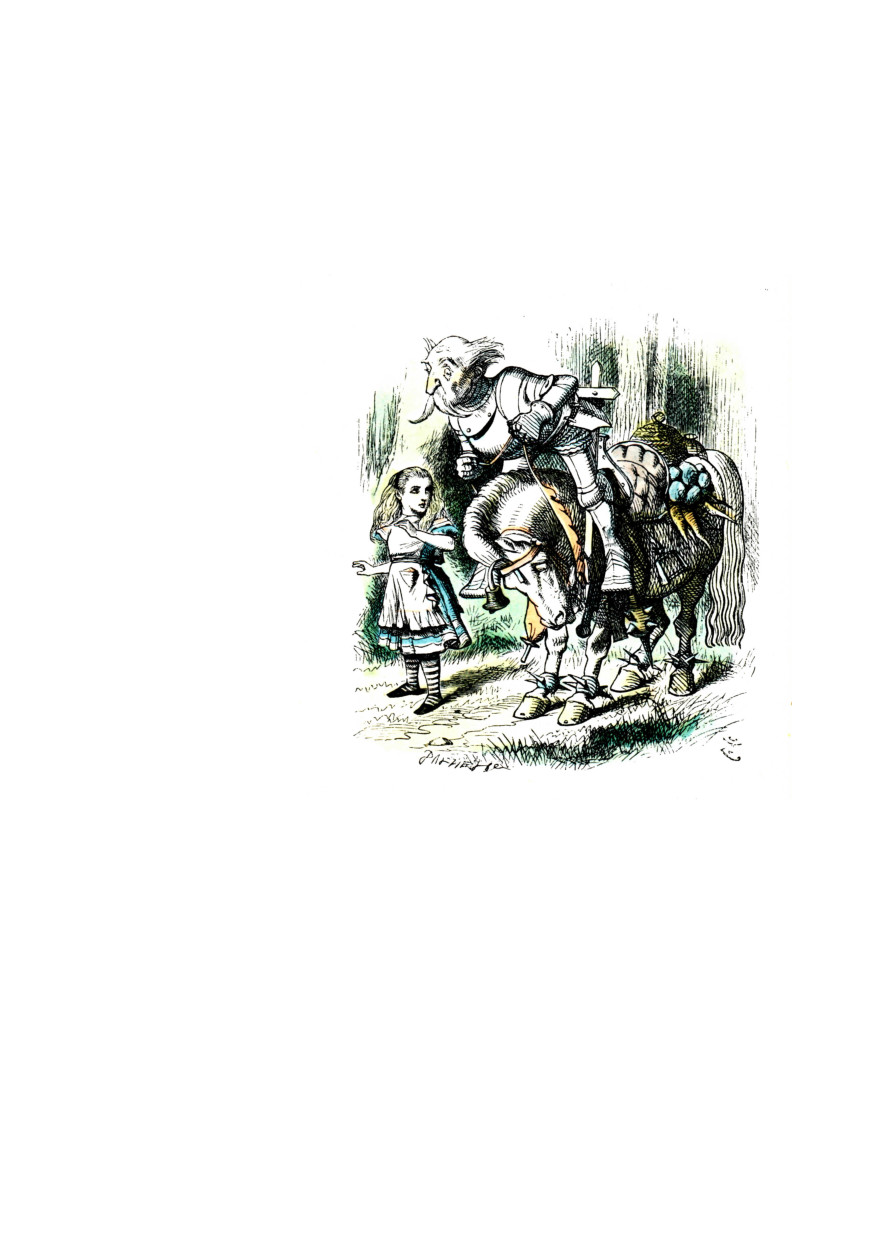
\includegraphics{img/Tenniel-Knight}}

\begin{quotation}
``I see you're admiring my little box,''  the Knight said in a
friendly tone. ``It's my own invention -- to keep clothes and
sandwiches in. You see I carry it upside-down, so that the rain ca'n't
get in.''

``But the things can get out,'' Alice gently remarked. ``Do you know
the lid's open?''
``I didn't know it,''  the Knight said, a shade of vexation passing over his face.

\begin{flushright}
\em -- Lewis Carroll, Through the Looking Glass\\
 illustrated by John Tenniel
\end{flushright}
\end{quotation}


\end{document}

